%%%%%%%%%%%%%%%%%%%%%%%%%%%%%%%%%%%%%%%%%%%%%%%%%%%%%%%%%%
\begin{frame}
\frametitle{Spark Components: System-level View}
%%%%%%%%%%%%%%%%%%%%%%%%%%%%%%%%%%%%%%%%%%%%%%%%%%%%%%%%%%
	\begin{figure}[h]
	  \centering
	  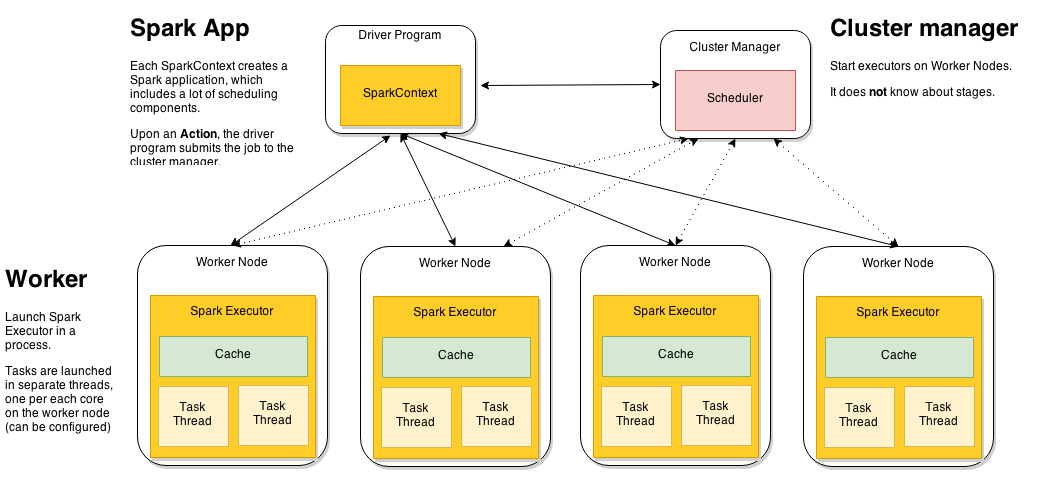
\includegraphics[scale=0.33]{./Figures/spark_system}
	  \label{fig:spark_components}
	\end{figure}
\end{frame}

%%%%%%%%%%%%%%%%%%%%%%%%%%%%%%%%%%%%%%%%%%%%%%%%%%%%%%%%%%
\begin{frame}
\frametitle{Spark Deployment Modes}
%%%%%%%%%%%%%%%%%%%%%%%%%%%%%%%%%%%%%%%%%%%%%%%%%%%%%%%%%%
\begin{itemize}
	\item {\bf The Spark Framework can adopt several cluster managers}
	\begin{itemize}
		\item \emph{Local Mode}
		\item \emph{Standalone mode}
		\item \emph{Apache Mesos}
		\item \emph{Hadoop YARN}
	\end{itemize}

	\vspace{20pt}

	\item {\bf General ``workflow''}
	\begin{itemize}
		\item Spark application creates \texttt{SparkContext}, which initializes the \texttt{DriverProgram}
		\item Registers to the \texttt{ClusterManager}
		\item Ask resources to allocate Executors
		\item Schedule Task execution
	\end{itemize}
\end{itemize}
\end{frame}

%%%%%%%%%%%%%%%%%%%%%%%%%%%%%%%%%%%%%%%%%%%%%%%%%%%%%%%%%%
\begin{frame}
\frametitle{Worker Nodes and Executors}
%%%%%%%%%%%%%%%%%%%%%%%%%%%%%%%%%%%%%%%%%%%%%%%%%%%%%%%%%%
\begin{figure}[h]
  \centering
  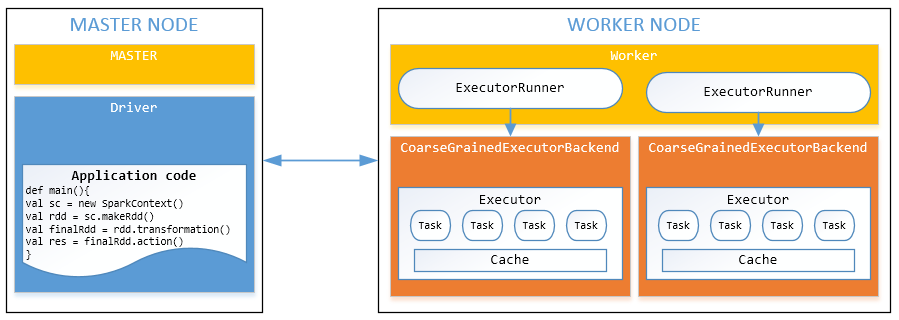
\includegraphics[scale=0.35]{./Figures/spark_worker_executor}
  \label{fig:spark_shuffle_sort}
\end{figure}

\begin{itemize}
	\item {\bf Worker nodes are machines that run executors}
	\begin{itemize}
		\item Host one or multiple \texttt{Workers}
		\item One JVM (= 1 UNIX process) per \texttt{Worker}
		\item Each \texttt{Worker} can spawn one or more \texttt{Executors}
	\end{itemize}

	\item {\bf Executors run tasks}
	\begin{itemize}
		\item Run in child JVM (= 1 UNIX process)
		\item Execute one or more task using threads in a \texttt{ThreadPool}
	\end{itemize}
\end{itemize}
\end{frame}

%%%%%%%%%%%%%%%%%%%%%%%%%%%%%%%%%%%%%%%%%%%%%%%%%%%%%%%%%%
\begin{frame}
\frametitle{Comparison to Hadoop MapReduce}
%%%%%%%%%%%%%%%%%%%%%%%%%%%%%%%%%%%%%%%%%%%%%%%%%%%%%%%%%%
\begin{columns}[t, onlytextwidth]
	\column[T]{.5\textwidth}
	{\bf Hadoop MapReduce}
	\begin{itemize}
		\item One Task per UNIX process (JVM), more if JVM reuse
		\item \texttt{MultiThreadedMapper}, advanced feature to have threads in Map Tasks
		\item[$\to$] {\bf Short-lived} Executor, with one {\bf large Task}
	\end{itemize}

	
	\column[T]{.5\textwidth}
	{\bf Spark}		
	\begin{itemize}
		\item Tasks run in one or more Threads, within a single UNIX process (JVM)
		\item Executor process statically allocated to worker, even with no threads
		\item[$\to$] {\bf Long-lived} Executor, with many {\bf small Tasks}
	\end{itemize}

\end{columns}

\end{frame}

%%%%%%%%%%%%%%%%%%%%%%%%%%%%%%%%%%%%%%%%%%%%%%%%%%%%%%%%%%
\begin{frame}
\frametitle{Benefits of the Spark Architecture}
%%%%%%%%%%%%%%%%%%%%%%%%%%%%%%%%%%%%%%%%%%%%%%%%%%%%%%%%%%
\begin{itemize}
	\item {\bf Isolation}
	\begin{itemize}
		\item Applications are completely isolated
		\item Task scheduling \emph{per application}
	\end{itemize}

	\item {\bf Low-overhead}
	\begin{itemize}
		\item Task setup cost is that of spawning a thread, not a process
		\item 10-100 times faster
		\item {\color{red} Small tasks $\to$ mitigate effects of data skew}
	\end{itemize}

	\item {\bf Sharing data}
	\begin{itemize}
		\item Applications cannot share data in memory natively
		\item Use an external storage service like Tachyon
	\end{itemize}

	\item {\bf Resource allocation}
	\begin{itemize}
		\item Static process provisioning for executors, even without active tasks
		\item Dynamic provisioning under development
	\end{itemize}
\end{itemize}
\end{frame}
